\begin{figure}[tb]
 \centering
 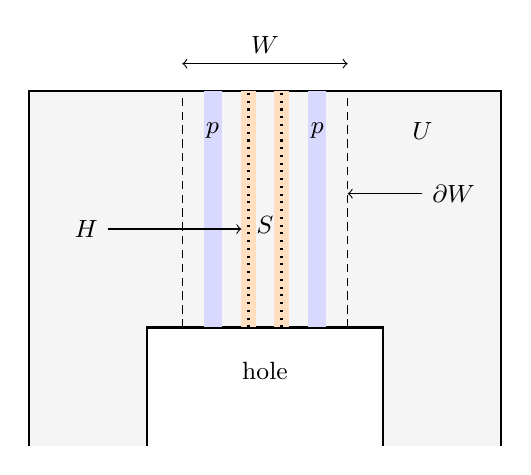
\begin{tikzpicture}[x=1cm,y=1cm,font=\small]
  \fill[gray!8] (-3,-1.5) rectangle (3,3);
  \fill[white] (-1.5,-1.5) rectangle (1.5,0);
  \draw[thick] (-3,-1.5)--(-3,3)--(3,3)--(3,-1.5);
  \draw[thick] (-1.5,-1.5)--(-1.5,0)--(1.5,0)--(1.5,-1.5);
  \fill[blue!15] (-.78,0) rectangle (-.55,3);
  \fill[blue!15] (.55,0) rectangle (.78,3);
  \fill[orange!25] (-.3,0) rectangle (-.12,3);
  \fill[orange!25] (.12,0) rectangle (.3,3);
  \draw[densely dashed] (-1.05,0)--(-1.05,3);
  \draw[densely dashed] (1.05,0)--(1.05,3);
  \draw[dotted,thick] (-.21,0)--(-.21,3);
  \draw[dotted,thick] (.21,0)--(.21,3);
  \node at (0,-.55) {hole};
  \node at (2,2.5) {\(U\)};
  \node at (0,1.3) {\(S\)};
  \node at (-.665,2.5) {\(p\)};
  \node at (.665,2.5) {\(p\)};
  \draw[->] (-2,1.25)--(-.3,1.25);
  \node[anchor=east] at (-2,1.25) {\(H\)};
  \draw[->] (2,1.7)--(1.05,1.7);
  \node[anchor=west] at (2,1.7) {\(\partial W\)};
  \draw[<->] (-1.05,3.35)--(1.05,3.35);
  \node[above] at (0,3.35) {\(W\)};
 \end{tikzpicture}
 \caption{A straight part of a strip \(S\) joining a hole to the
 outer free wall. Dotted lines indicate the interfaces cut to isolate
 \(S\). The pin region \(H\), shown along both interfaces, contains
 every endpoint of every lattice edge crossing either interface.
 The two
 guard bands \(p\) separate them from the artificial boundary of the
 wider patch \(W\). All bands have positive widths and positive
 intervening gaps. Parallel collars give the same separation at
 rectilinear turns. The bottom ends of the outer boundary and hole
 are omitted from the schematic.}
 \label{sectors:slit-figure}
\end{figure}
